\section{Implementation}

\subsection{Build plan}

\subsubsection{Background}

Any project centered around musicians or their instruments cannot avoid the term ‘feel’. Unlike math or physics where the goal is to arrive at a concrete and unified solution, music is often abstract and expressed through emotions or feelings. There are certainly wrong answers in music, but very few objectively correct answers, and this concept plays a huge role in how musicians choose their instruments.

\begin{figure}[h!]
  \centering
  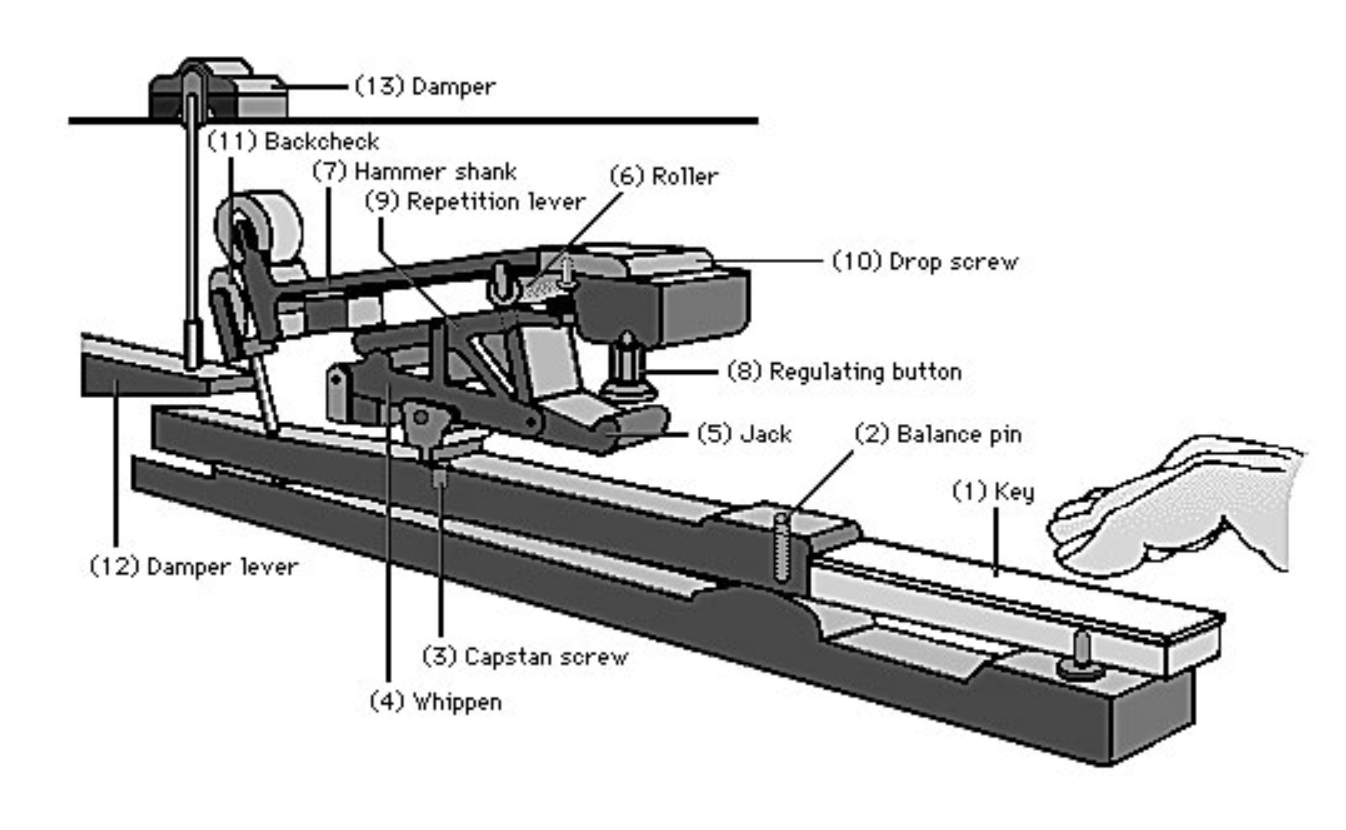
\includegraphics[width=\linewidth]{image/KeyMechanism.png}
  \caption{}
  \label{fig:key_mechanism}
\end{figure}

In a perfect world, the keys of any digital piano (also known as an electric keyboard, keyboard, or synthesizer) would feel, function, and look like an acoustic keyboard: if a player chooses to play a synthesizer, they have most likely played on an acoustic piano. Most keyboard players know that the tactile response of a key in any piano or synthesizer is important because it determines how each note reacts to the player’s touch. For example, lighter keys will respond more quickly to the touch, but will reduce the ease of creating a dynamic range in strike velocity compared to their heavier counterparts. Velocity-sensitive tension spring keys will provide a more uniform tension throughout the keystroke, while weighted keys are balanced on a “balance pin” that separates the user from its striking mechanism, shown in \textit{Figure \ref{fig:key_mechanism}}, and as a result varies in normal force as the key is pressed.

In addition, each performer and use of the instrument plays a role in determining the desired preference of key feel. EDM or heavily synthesized music designers will care less about key feel because most of the work in writing this type of music, besides determining the melodic structure, will come in post production and adjusting the key inputs from the computer. On the opposite end of the spectrum, classically trained musicians will dramatically care about key feel because most of the work is dedicated to how they express the music through their performance.

\begin{figure}[h!]
  \centering
  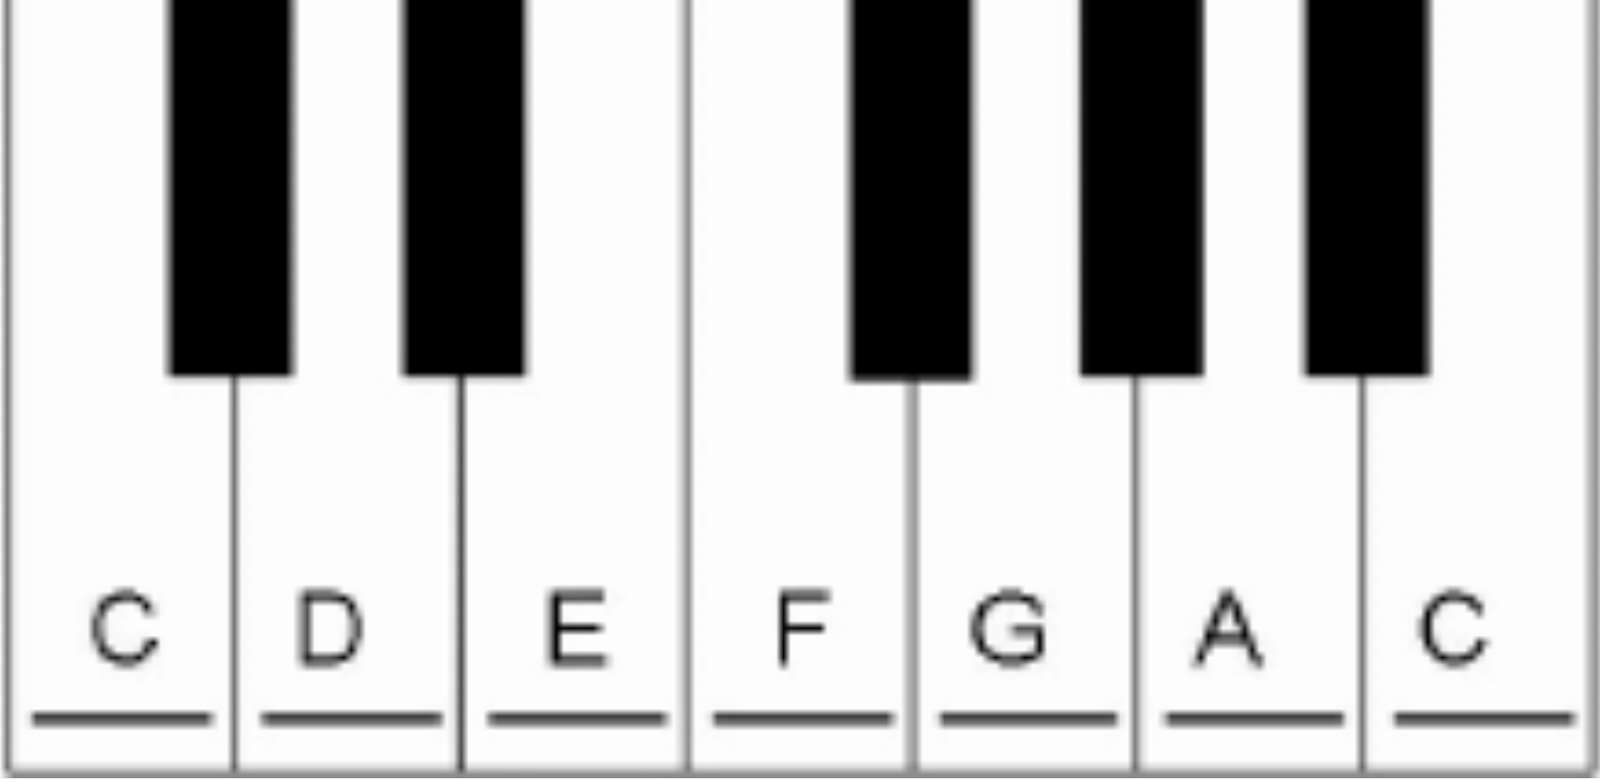
\includegraphics[width=0.5\linewidth]{image/Octave.png}
  \caption{}
  \label{fig:octave}
\end{figure}

On top of the key feel, the amount of keys available to the player has its own important role to the user and their desired end goal as well. To gather a better understanding, a single octave on a piano consists of twelve keys: seven white keys, and five black keys as shown in \textit{Figure \ref{fig:octave}}. A writer who is focused on beat making and synthesized music can craft most of their music with a single octave and the use of transposing that octave. A writer who is classically trained will most likely be adjusted to a standard 7 octave keyboard without the option of transposition. Weary of what will be possible for us, we used this information and decided our device should be modeled similarly to a professionally designed MIDI controller that is smaller than five octaves to keep the portability, but larger than one octave to provide a useful range to most players.

\subsubsection{Key Size}
Our key design was created by referencing two different electric keyboards: the \textit{Roland DP-90} and \textit{Arturia’s Keylab MkII - 61 key}. We chose to take our initial key measurements from these devices because our group has direct access to these and there are no official standardized key sizes. Although \textit{Figure \ref{fig:octave}} does not express the nuances in key design, there are six different key shapes that we have labeled: black, b, t, d, tb, and td, from the letter shapes they are most similar to. tb and tb are a hybrid of the t and b or t and d shape keys. The measurements taken from those devices are shown in \textit{Table \ref{Tab:key_dimensions}} .

\begin{table}[]
  \centering
  \resizebox{\textwidth}{!}{%
  \begin{tabular}{|l|l|l|l|}
    \hline
    Keyboard                & Roland DP-90 & Keylab MkII & Our Choice \\ \hline
    Black Key               &              &             &            \\ \hline
    Base Width (mm)         & 12           & 12          & 12         \\ \hline
    Base Length (mm)        & 95           & 80          & 80         \\ \hline
    Top Width (mm)          & 9            & 9           & 9          \\ \hline
    Top Height (mm)         & 88           & 72          & 72         \\ \hline
    Standard White          &              &             &            \\ \hline
    Base Width (mm)         & 22           & 22          & 22         \\ \hline
    Base Length (mm)        & 150          & 130         & 130        \\ \hline
    b cut-in (mm)           & 9            & 8           & 8          \\ \hline
    t cut-in (mm)           & 4.5 / 4.5    & 4 / 4       & 4 / 4      \\ \hline
    d cut-in (mm)           & 9            & 8           & 8          \\ \hline
    tb cut-in (mm)          & 3 / 6        & 3 / 6       & 3 / 6      \\ \hline
    td cut-in (mm)          & 6 / 3        & 6 / 3       & 6 / 3      \\ \hline
    Key Separation (mm)     & 1.5          & 2           & 2          \\ \hline
    Trigger Angle (Degrees) & 6.972        & 8.296       & 5          \\ \hline
  \end{tabular}}
  \caption{}
  \label{Tab:key_dimensions}
\end{table}

Our objective is to empower any creative or independent writer, so these devices were happily chosen in particular for their difference in range of use cases. The \textit{Roland DP-90} is designed such that it “performs and responds like a grand piano”, while the \textit{Keylab MkII} is designed as a “definitive MIDI controller keyboard ... a luxurious, expressive tool for your studio” . By taking measurements from two vastly different devices and noticing the minimal variation between their two key sizes, we were able to be confident that our key size choice would suffice. For the project, we chose to go with the cut-in and general measurements of the \textit{Keylab MkII} because the distance between each key was about 2 mm, compared to the 1.5 mm distance the \textit{DP-90} keeps. Since this project will be crafted without professional business assistance, we felt as much leeway to avoid collisions as possible would be beneficial. Additionally, we felt that using the smaller dimensions in key sizes would help reduce the overall form factor of the device and keep it as portable as possible.

\subsubsection{Number of Keys}

We chose to create a thirty-two key keyboard. We landed on this choice as a result of the following factors: first, when this device is in use we do not wish to limit our users to one octave. Our autocomplete AI is modeled from classical music and we understand that the input and output melodies will likely span over a wider range than one octave. We also recognize that this device is more useful in the post-production setting compared to a performance setting and therefore does not need the full seven octave range. Second, to keep the cost low and the form factor small, we wanted to keep the keys below three octaves. We are choosing to build this keyboard as a portable, stand-alone, robust piece of equipment and we believe our device should not cause struggle to carry around. With the measurements we took, each octave will accompany about 262 mm (10.315 inches) of space in keys alone. This means a thirty-two key keyboard is estimated to need 666 mm ($ \approx $ 2.185 ft) of lateral space in keys alone. We knew when multiplexing our signals that using a power of two for our set of inputs would be beneficial. A power-of-two inputs allows us to use the entirety of each multiplexor we implement. As a result, thirty-two keys provides a set of two and a half octaves and will utilize the entirety of each multiplexor without extending the keyboard to sixty-four keys, which is around five octaves. To compare, sixty-four keys would extend to 1290 mm ($ \approx $ 4.232 ft) and in our humble opinion, would no longer allow this device to be comfortably portable.

\subsubsection{Key Functionality}

In our application we are looking to distinguish which note is being pressed, the velocity that note was triggered, and which channel the device is communicating through. With the digital functionality of the key in mind, the physical key design only has to worry about how to communicate the velocity of the note to the Arduino, which will later be sent to the Pi. To be able to do this, we are using a two button trigger system for each key. As observed in \textit{Figure \ref{fig:key_mechanism}}, there are two rods extending from the bottom of the key of different lengths. In the full keyboard model, these rods are lined up with two silicone covered buttons, one of which is triggered at the start of the keystroke and the other is triggered near the conclusion of the keystroke. The difference in trigger time between the two buttons will determine the note velocity which is explained in greater detail from Section IDK YET .

After basic functionality, our next concern is key feel. With the time allotted for this project, what is possible to craft at this level of expertise, and our desire for ease of portability, it is obvious from observing \textit{Figure \ref{fig:key_mechanism}} that we will not attempt to replicate the full counter-weighted key design. To keep costs low and durability high, we are also avoiding any semi-weighted keys or the usual expensive key material such as ivory or wood. By utilizing 3D printed plastics, we are able to create custom, robust designs at a cheaper cost than the alternatives.

    INSERT COST OF MATERIAL AND STRENGTH OF MATERIAL TABLE

To provide the actuation action for the key itself, we will be using tension springs to hold the key in place as it sits on a lever.

\subsection{Prototyping}

\subsubsection{Keyboard}

Before deciding the selection of tension springs, actuator lengths, and the peripheral components to complete the key functionality, we decided that an initial design should first be created and printed to ensure our future endeavors would work as planned. With 3D printing, especially while utilizing an ‘at home’ 3D printer, there are a few parameters we need to keep in mind.

\begin{figure}[h!]
  \centering
  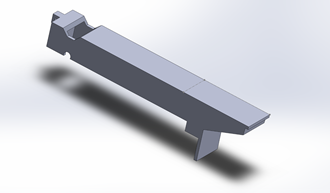
\includegraphics[width=0.7\linewidth]{image/WhiteModel1.png}
  \caption{}
  \label{fig:white_model1}
\end{figure}

An associate of the team built the 3D printer we will be putting to use. Due to the years of development, custom embedded code, and a variety of parts from different manufacturers, the best resource to learn about the printer would be our associate himself: Anton Strickland. Anton’s printer was initially purchased as a Creality Ender 5. The first major change to the hardware was the replacements of the control board from an eight bit control board with fifteen kilobytes of memory to a thirty-two bit control board the 512 kilobytes of memory. The increase in processing power along with the increase in memory allows for some advanced features such as enhanced acceleration control, jerk reductions, and square wave output.

The enhanced acceleration control as well as the jerk reduction are important parameters for the speed of the print. We will be sharing this printer with other groups and since we plan to print possibly more than thirty-one keys, the key rail configurations, and the electronics housing, it is important to make sure the prints will be executed accurately and produced in time to be added to the prototype. The enhanced acceleration control allows the device to change velocity with more precision and boost our confidence to ramp up the speed of the print where at all possible. As a result of attempting more speedy prints, the jerk, or change in acceleration, needed to be monitored more greatly as well. With the new control board, reducing the jerk and altering the extrusion rate of the filament with the newly enhanced parameters is finally possible. In addition to these parameters, the new board can signal using square waves as an output. This means the data that we are sending and monitoring is more consistent and reliable. All together, this means faster prints with a smaller rate of failure compared to the previous board.

In addition to the hardware that boosts the software, this device is equipped with 2209 Stepper motor drivers which replaced the original drivers to add more smooth and consistent nozzle travel. The nozzle has also been replaced with an upgraded hot end titanium heatbreak nozzle that is designed to prevent heat creep. This is important when printing multiple prints in rapid succession to prevent any overheating or inconsistent filament extrusion. This also means that the printer can print twenty-four hours a day and seven days a week without a high risk of print failure.

The hardware Z-axis lead screw has also been replaced from four-hundred steps per millimeter to 1600 steps per millimeter, increasing the accuracy of layer size and decision variation. This device can print anything smaller than 220x220x400 mm, a line width that can be altered from .2 mm to .8 mm with as small as +/-.15 mm tolerance, and customizable infill percentages.

From this information, it is evident that most prints with any structural integrity will be indefinitely feasible as long as each print is smaller than the allotted max size of 220x220x400 mm.

To begin crafting the keys for this device, I started with a basic model I have labeled textit{WhiteKeyStart.SLDPRT}, shown in \textit{Figure \ref{fig:white_model1}}. The white keys, also known as natural keys named after the not sharp nor flat notes in music, are the larger set of keys which make up most of the space on the keyboard. As you can see from \textit{Figure \ref{fig:white_model1}}, this key does not have the actuating levers to connect to the buttons on the PCB nor does it have any cuts to make room for the black keys, or non-natural keys, which fit in-between most of the white keys. This model was crafted from measurements and observations made from \textit{Table \ref{Tab:key-dimensions}} and is the baseline of each natural key model. Looking at the model in \textit{Figure \ref{fig:white_model1}} closely, one can observe the incomplete sketch line that is about one-third into the key. This sketch marks the location where each key needed to be cut, forty-eight millimeters from the base, to create the five different models of the natural keys and ultimately allowed the crafting of the following models to be much easier.

The major parameters of this model are as follows. Each natural key has a base width of twenty-two millimeters and a playable length of 123.71 mm which is a little shorter than the measured length of the Keylab MkII, but fits the idea of the project due to our desire to create a portable device. Viewing \textit{Figure \ref{fig:white_model2}}, there is a two millimeter lip on the end of the key, shown in the top right of the figure, to the correct key feel and provide the user with better feedback to distinguish the tip of the key. Below that lip is a five millimeter drop at a 95 degree angle, followed by a 20 degree 28.73 mm drop to provide aesthetic distance from the lip and preventing the key from looking blocky from the front.

Next we can see the functional aspects of the design. Below the 28.73 mm 20 degree decline is a 22 mm guiding plane that is two millimeters thick. This serves not only as a guiding plane, but also prevents the user from viewing the hidden electronics beneath the key. 15 mm up from the bottom of the guiding plane is a 10 mm long platform that is used to limit the actuation of the key for a realistic ten degree actuation angle which will become more apparent in the full model.

\begin{figure}[h!]
  \centering
  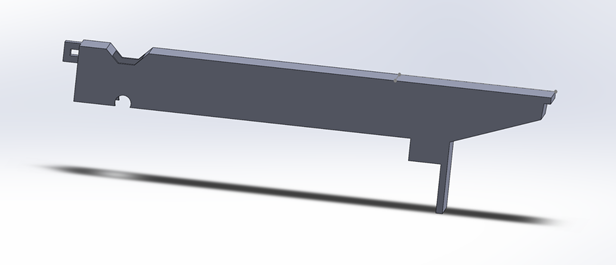
\includegraphics[width=0.8\linewidth]{image/WhiteModel2.png}
  \caption{}
  \label{fig:white_model2}
\end{figure}

In the first iteration, the almost complete circle to the far left is five millimeters in diameter. This will be touched on later in this design section of the document. Above that circle is a divot, in the shape of an upside trapezoid, five millimeters at the base with 45 degree inclines to the top of the key. This divot is used to allow the cover of the keyboard to not only keep help guide the key and keep it in place, but also to once again prevent the user from clearly seeing the electronics hidden inside the full device. Finally, on the far top left of the key is a 3x2x5mm hole designed to hook onto the tension springs that help provide the pull-back of the actuation. Each natural key has the exact same cut-in values as given in \textit{Table \ref{Tab:key_dimensions}}.

Next in the first iteration of key designs is the non-natural key, or black key, named after the sharp and flat notes these keys trigger. From a design standpoint, it is helpful that all of the non-natural keys share the same structure. To begin, the guiding plane and size of the connecting platform have the same measurements of the natural keys, fifteen millimeter plane and a ten millimeter platform. The divot, the hole beneath the divot, and the extruded cut where the spring attaches all have the same measurements as the natural keys as well. The original design has a playable length of 120.71 mm. Due to the shorter playing length and same guiding plane length, the actuation of the keys has been approximated to be around 15 degrees, compared to the 10 degree actuation of the natural keys. This key does not need any tip as a tip could obstruct any transition the player may have switching from the non-natural keys to the natural keys, instead the tip of the non-natural key has a 15 degree chamfer on all sides to allow the fingers to slide from the elevated top of the non-natural key to the lower natural keys. As a result, the top of the key is thinner than the base, as is expected from the measurements taken in Table 1. To gather a better understanding, the base of the key is the section which aligns with the elevation of the natural keys, while the tip elevates ten millimeters above the key. Between the base and the tip is what makes up the key itself.

\begin{figure}[h!]
  \centering
  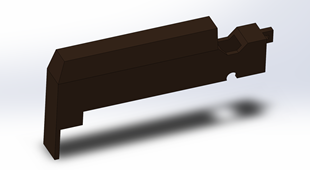
\includegraphics[width=0.7\linewidth]{image/BlackModel.png}
  \caption{}
  \label{fig:black_model}
\end{figure}

The first iteration of the key rail and base was intended to be a completely 3D printed component shown in \textit{Figure \ref{fig:base_model1}}. This rail and base, filed as KeyRail2.SLDPRT, features a five millimeter thick base for structural integrity with an overall length of 94.5 mm to allow the guiding plane of the natural keys to sit in front of the base itself. The six millimeter extruded cuts, which occur 76.5 mm from the back of the base, are to allow the guiding planes from the black keys to slot within the holes freely and without obstruction. There is a 10 degree incline at the front of the base and a 10 degree incline near the non-natural key guiding holes, which is addressed later, to give the keys a flat plane to stop the actuation when the keys are fully pressed to play. The rail that the keys attach to, which is raised 27.83 mm from the back of the base to the center of the rail, is 4.85 mm in diameter and has two millimeter plastic spacers at appropriate distances to slot each key into position while allowing enough space to easily actuate. In this design, I allowed one millimeter of tolerance for each key. This rail is supported by 2.5x2mm thick vertical poles with a 2.5x3 mm horizontal piece of support plastic. When assembled, the full first prototype can be seen in \textit{Figure \ref{fig:assembled_model}}.

\begin{figure}[h!]
  \centering
  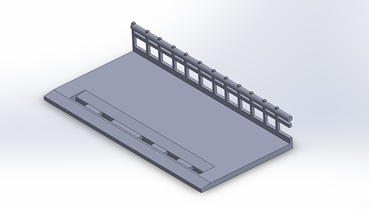
\includegraphics[width=0.8\linewidth]{image/BaseModel1.png}
  \caption{}
  \label{fig:base_model1}
\end{figure}

To allow an appropriate prototype test, I first chose to simulate the assembly with collision detection enabled. Luckily, while all keys were in their starting position, no collisions were detected. Sadly, when some keys were actuated, the simulate responded with a collision report. It was difficult, at first, to determine where the collisions were occurring. In some settings, it was evident that certain collisions only occurred when the keys were placed in positions that would not be possible in the final assembly and actual implementation of the device. In other cases, the collisions could not be easily seen in the model. Due to this, I decided to run a test print of some of the pieces present. I figured I would not need the entire model to determine where the problems were occurring as the difference in model pieces were not drastic.

\begin{figure}[h!]
  \centering
  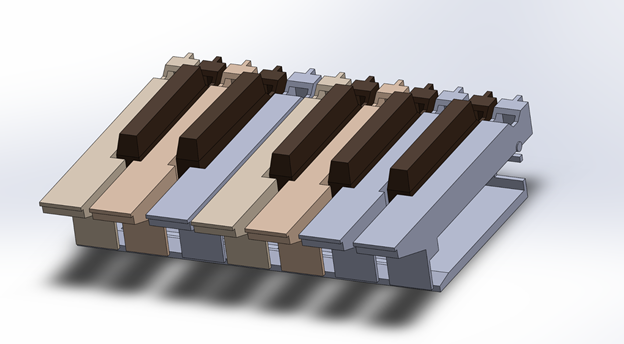
\includegraphics[width=0.9\linewidth]{image/AssembledModel.png}
  \caption{}
  \label{fig:assembled_model}
\end{figure}

\textbf{Iteration One}

This first print was a test to determine the functionality of the keyboard in its preliminary stage. As the reader can tell by the title listed at the beginning of the document, there are no mechanical engineers on this team and therefore there are no members with a solid grasp on tolerances for different applications. We figured the best way to determine the tolerance we are looking for is to test a couple different sizes. In the test print, the rail itself was designed to be 4.85 mm in diameter, so obviously we needed to allow the circular cut which rests on the rail to be larger than 4.85 mm in diameter. For this print, we used the rail, the b-model, the t-model, and two non-natural keys. The b-model had a circular cut of 5.35 mm in diameter, the t-model had a circular cut of 5.15 mm in diameter, and the black keys had a circular cut of 5 mm in diameter shown in \textit{Table \ref{Tab:connections}}.

\begin{table}[]
  \centering
  \begin{tabular}{|l|l|}
    \hline
    Model           & Connection Diameter (mm) \\ \hline
    Rail            & 4.85                     \\ \hline
    b-model         & 5.35                     \\ \hline
    t-model         & 5.15                     \\ \hline
    Non-natural key & 5                        \\ \hline
  \end{tabular}
  \caption{}
  \label{Tab:connections}
\end{table}

The results of the model are shown in \textit{Figure \ref{fig:print1}} below.

\begin{figure}[h!]
  \centering
  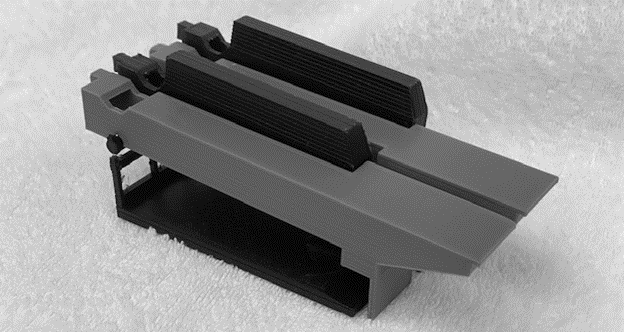
\includegraphics[width=0.8\linewidth]{image/Print1.png}
  \caption{}
  \label{fig:print1}
\end{figure}

At first glance, the model seemed really well produced. The results of the different tolerances for the connecting circular cut to rail are as follows. With a .15 mm tolerance, as exemplified from the non-natural keys, the keys snapped into place and connected with the keyrail. At a .3 mm tolerance, the t-key was able to slide, but with resistance. At a .45 mm tolerance, the b-key was able to slide with ease. Luckily, the .45 mm tolerance did not make the b-key feel shaky or disconnected from the rail which was an issue we hoped to avoid and learn about through this test. From this test, we knew that moving forward with a .45 mm tolerance was our best bet. The major issue with this test is that the rail itself is not perfectly round because it is constructed of linear layers and, although it provides a good idea for the final model, is not the best example of how rotational tolerances should be designed. This is addressed in Iteration Three of the prototype.

\begin{figure}[h!]
  \centering
  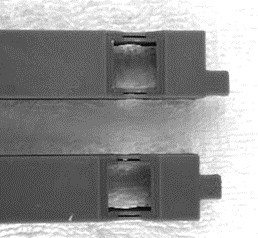
\includegraphics[width=0.6\linewidth]{image/Print2.png}
  \caption{}
  \label{fig:print2}
\end{figure}

After toying with the model for some time, a few issues were brought to light. The most obvious being the uneven slots designed to grip the tension springs, shown in \textit{Figure \ref{fig:print2}}. Since we did not change the base location of the holes to hook the springs, the way the cuts were made created uneven spacing of the aft tip of the key. Not only that, with the holes using 2 mm of wall space and being 5 mm deep, it was evident after the print that those holes needed to be less deep to actually allow the spring to hook. Since the keys are light and the tension of the spring does not need to be exceptionally tight or forceful, it will be more than possible to reduce this thickness without any major issues in functionality.

\begin{figure}[h!]
  \centering
  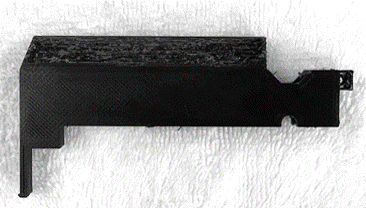
\includegraphics[width=0.8\linewidth]{image/Print3.png}
  \caption{}
  \label{fig:print3}
\end{figure}

The next minor fault was with the quality of the print. Due to the chamfered edges of the non-natural keys and the way the model was designed, the key needed support material between the base and the tip of the key. This support material, when removed, caused a rough edge to the key itself, shown in \textit{Figure \ref{fig:print3}}.  To fix this, our team debated a few different ideas. First, we thought about restructuring the key itself and removing the chamfer such that the key could print in a different orientation. This would be additionally helpful because it would allow the key to be printed from the top of the key down, meaning the top plane would be placed on the printing bed leading to a smoother key texture where the user plays. The biggest downside to this idea is that the key would lose its gradual shape from the top of the key and make the key itself look and feel more blocky to the player.

An alternate idea, rather than changing the model, is to simply add a thin layer of epoxy resin to the surface of the key to create that smooth key feel the player will desire. This eliminates the option of a blocky key, but also adds additional work on our end and may cause an uneven surface finish. Another alternative idea is to manufacture these non-natural keys at a professional 3D printing company. This idea has already been debated by the team before the model was even completed, but comes with its own problems of shipping time and extra cost. These alternatives will be discussed and finalized in SECTION IDK YET.

Continuing with the non-natural key, another issue reared its ugly head: actuation interference. Since the non-natural keys were designed to be only 3 mm shorter than the natural keys, the natural keys were unable to actuate fully without coming in contact with the guiding plane of the non-natural keys and stopping the actuation of the natural keys. The length of one or the other needed to change and this is discussed in Iteration Three of the prototype.

Another issue we discussed is the fact that there were no parameters in place to prevent the key from actuating backwards. Considering the tension spring will be pulling the key in place, we needed to take into account the possibility that the resting position of the spring will most likely not be the exact distance from the two hooks in the final design. And that we may not even want the resting position of the spring to be of equal length of the two hooks the spring will attach to. This is further touched on in Iteration Three of the prototype.

\begin{figure}[h!]
  \centering
  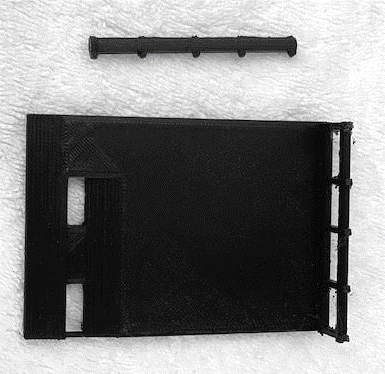
\includegraphics[width=0.8\linewidth]{image/Print4.png}
  \caption{}
  \label{fig:print4}
\end{figure}

The final issue, as shown in \textit{Figure \ref{fig:print4}}, is the poor structural integrity of this completely 3D printed part. Within two hours of the print being completed, the rail detached from the support material rendering the entire print useless. Luckily we were able to receive the results from the test that we needed before the entire print broke down. While discussing the integrity and viewing \textit{Figure \ref{fig:print4}}, it is also evident that creating overhangs that this model demands results in a lot of stringing and print mutations that were not intended.

Thus, it was back to the drawing board, or as SolidWorks users describe, the sketching board, and back to redesigning

One major benefit of this print is noting that an estimated time of printing all thirty-one keys is about two days or 49 hours. Anton, my reference for the printer, states that this can be sped up to about 42 hours for all thirty-one keys if necessary. Due to the alterations made to the printer, this can be a 42 hour print straight through with only adding extra time to remove the print from the bed. This indicates that there will be zero issues regarding timing when it comes to our prints considering we have approximately three months to print and assemble this device.

\textbf{Iteration Two}

As the reader may notice, there are many references from the first iteration to the third iteration. This is because iteration two did not have many major changes, was quickly discussed, and transformed into Iteration Three which is as follows.

\textbf{Iteration Three}

From the results of Iteration One and Iteration Two we decided to alter the length of the non-natural keys to prevent actuation interference between the non-natural and the natural keys. In this design, the non-natural key is 72 mm in base length and 69 mm in tip length. Although this design decreases the length of the non-natural key by about 10%, we figured this difference would not be an issue as there are no standardized key lengths and this is a collegiate level project. Obviously the base and key-rail design needed to account for this change, but this is not the only change which helped develop this model into the third iteration.

\textit{Figure \ref{fig:base_model3}} shows the file KeyRail3b.SLDPRT. It is obvious when compared to the first iteration that many changes occurred. The comparison of the two versions can be seen in \textit{Figure \ref{fig:base_model2}}.

\begin{figure}[h!]
  \centering
  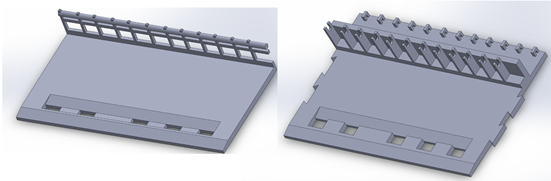
\includegraphics[width=0.8\linewidth]{image/BaseModel2.png}
  \caption{}
  \label{fig:base_model2}
\end{figure}

The first major change in iteration three compared to that of iteration one is the absence of a key rail. After witnessing the performance of the 3D printed rail and noticing the deformities and the overhangs, we decided to completely eliminate the idea of a 3D printed rail. Instead of a printed rail we are choosing to purchase a stainless steel rod which is discussed in the Component Selection section of this document. By eliminating the rod from being printed we are able to not only utilize a smoother rod to create smoother actuation, but also allow the model to be printed from the base up with only one overhanging section: the spring hook slots. From the model of the natural keys and its test print, however, we know we do not need to worry about these overhangs as they are similar overhangs presented in that model. This is shown in \textit{Figure \ref{fig:print5}}.

\begin{figure}[h!]
  \centering
  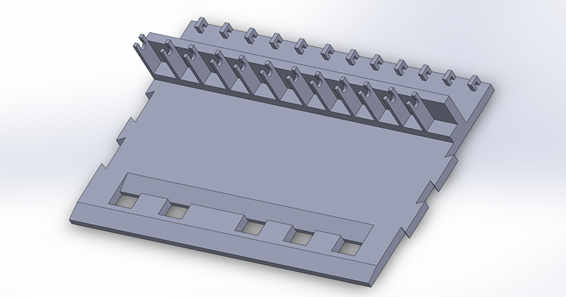
\includegraphics[width=0.9\linewidth]{image/BaseModel3.png}
  \caption{}
  \label{fig:base_model3}
\end{figure}

Furthermore, discussing the width of the holes for the springs to attach, we have reduced the width from five millimeters to 2.5 mm on both the keyrail base and the keys themselves. This thinner design will allow the springs to hook around the plastic, through the holes, and prevent slipping of the springs. From the test which we observed the different tolerances of the key rail connection to the keys, we have decided to allow a .15 mm diameter tolerance for the metal rod to snap into the chassis. This model, seen in \textit{Figure \ref{fig:base_model3}}, also features a 5 mm wide platform raised 21.83 mm from the base behind the rail itself to prevent the key from rotating past the horizontal plane in the opposite direction. We also changed the support which holds the rod from a 2.5x2 mm pole to a 2x8 mm pole to increase structural integrity. Although, when viewing the keyboard from the players perspective, there is less support in the x axis for these poles, there is significantly more support in the z direction which is where more of the force of the player will be applied. In addition, because we are using a stainless steel rod in the x direction, our device should have more than enough support to operate under normal playing conditions easily.

\begin{figure}[h!]
  \centering
  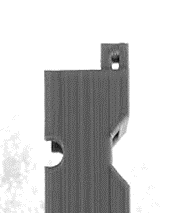
\includegraphics[width=0.25\linewidth]{image/Print5.png}
  \caption{}
  \label{fig:print5}
\end{figure}

Continuing to discuss \textit{Figure \ref{fig:base_model3}}, the non-natural key incline next to the guiding holes has been altered to 15 degree to better account for the angle of actuation those keys will encounter. We also increased the hole width from 6 mm to 10 mm to provide ample room for the guiding plane on the black to actuate through. Increasing this hole size was also only possible by shortening the key size of the non-natural key and allowing 2.75 mm of 5 mm thick support between the guiding holes for the non-natural keys and the start of the key rail’s base incline for the natural keys.

The final major change shown in \textit{Figure \ref{fig:base_model3}} are the odd protrusions and extruded cuts on the far left and right of the base. After reviewing the printing size limitation of 220x220x300 mm, we knew we could not print the entire keyboard base at once as one octave alone is 192 mm in width and we aim to have a 2.5 octave keyboard. To combat this, we decided to create a design such that the different base pieces could attach like a puzzle. After these pieces attach, we plan to glue the model together using a ‘3D print-safe’ adhesive and attach a thin vinyl layer to the bottom of the base to create a more professional look.

\begin{figure}[h!]
  \centering
  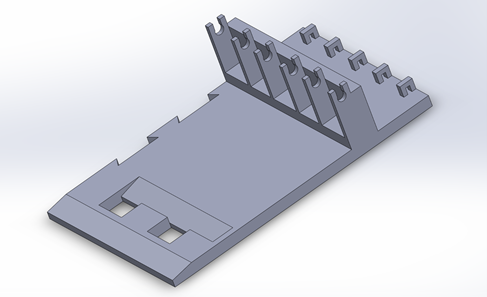
\includegraphics[width=0.8\linewidth]{image/BaseModel4.png}
  \caption{}
  \label{fig:base_model4}
\end{figure}

Since we are creating a keyboard that is two and a half octaves wide, we also need to create a model for the half octave keyrail shown in \textit{Figure \ref{fig:base_model4}}. This model shares the same measurements as the other keyrail and base model, but terminates at the fifth key’s support beam.
The other change made after observing the print was manually centering the hook hole for each one of the key models. This is shown in \textit{Figure \ref{fig:key_models}}.

\begin{figure}[h!]
  \centering
  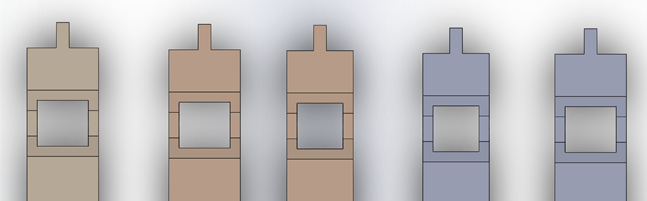
\includegraphics[width=0.8\linewidth]{image/KeyModels.png}
  \caption{}
  \label{fig:key_models}
\end{figure}

After testing and reiterating the initial print models, we were finally able to move on to the body of the keyboard itself. Much like the previous prints, we now realized the importance of being able to print from one face up with zero overhangs and this is something we achieved. We also knew our limitation from the printer itself and therefore, the body model is as follows. We needed an elevated base to allow the keys to actuate, a group of printed parts that follow our restrictions as well as attach together, and an area to house the electronics and display.

\begin{figure}[h!]
  \centering
  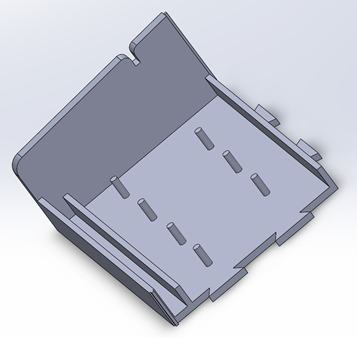
\includegraphics[width=0.8\linewidth]{image/BodyModel1.png}
  \caption{}
  \label{fig:body_model1}
\end{figure}

For the front left base body print we created the model shown in \textit{Figure \ref{fig:body_model1}}. From the player’s perspective, at the very front is a 31 mm tall wall, followed by an 11 mm gap, and then a 16 mm tall wall. This is to help guide the natural key’s actuation and prevent the player from seeing the electronics within the device. It is also a standard set up that most portable electric keyboards have. Within the center are seven poles, each 16 mm tall, and a 16 mm tall wall in the back. Each 16 mm high structure was designed to hold the keyrail above the base, shown in \textit{Figure \ref{fig:body_model2}}, which allows each key the space it needs to actuate. The front and side walls are also equipped with a 1 mm protrusion along the vertical axis of the inner wall, and protrusions similar to that of puzzle pieces to all each section to easily be connected and glued together.

\begin{figure}[h!]
  \centering
  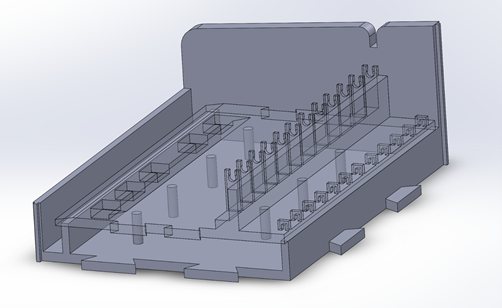
\includegraphics[width=0.8\linewidth]{image/BodyModel2.png}
  \caption{}
  \label{fig:body_model2}
\end{figure}

As can be seen in \textit{Figure \ref{fig:body_model2}}, the key rail, base, and body fit together perfectly, allowing space in the front for the guiding plane of the natural keys.

To the left of the base we see a divot that is 4 mm wide at a variable depth. This divot is to allow the cover to sit comfortably on the full assembly without sliding off. The bases of each model is 5 mm from the ground up. The front and inner wall are 4 mm, while the outside walls are all 8 mm thick to provide a robust shell for the device. Also, from \textit{Figure \ref{fig:body_model2}}, we can see that the puzzle-piece like protrusions do not align from the base to the body. This was intentional to produce a more rigid structure when the device is fully assembled.

\textbf{Assembly}

The full keyboard is about 483 mm wide, 322 mm deep, and 93.89 mm tall. From our printer restrictions of 220x220x300 it is obvious we cannot print this as one full device. To counter the limitations, we divided the keyboard into six different sections in the style of a 2x3 matrix. For our design, the first row is dedicated to the electronics housing and the second row is dedicated to the keys. The body pieces which make up this arrangement are shown below. In \textit{Figure \ref{fig:body_parts}(a)}, we have the 1x1 body piece, in \textit{Figure \ref{fig:body_parts}(b)}, we have the 1x2 body piece, in \textit{Figure \ref{fig:body_parts}(c)}, we have the 2x1 body piece, in \textit{Figure \ref{fig:body_parts}(d)}, in \textit{Figure \ref{fig:body_parts}(e)}, we have the 1x3 body piece, we have the 2x2 body piece, and in \textit{Figure \ref{fig:body_parts}(f)}, we have the 2x3 body piece.

\begin{figure}[h!]
    \centering
    \begin{subfigure}[b]{0.45\textwidth}
      \centering
      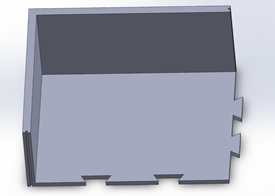
\includegraphics[width=\textwidth]{image/BodyModel3.png}
    \end{subfigure}
    \begin{subfigure}[b]{0.45\textwidth}
      \centering
      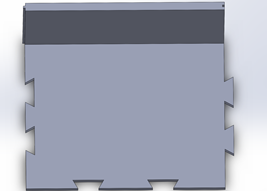
\includegraphics[width=\textwidth]{image/BodyModel4.png}
    \end{subfigure}
    \begin{subfigure}[b]{0.45\textwidth}
      \centering
      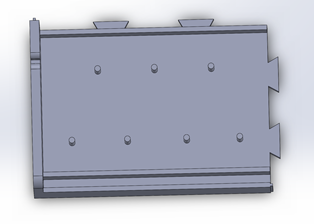
\includegraphics[width=\textwidth]{image/BodyModel5.png}
    \end{subfigure}
    \begin{subfigure}[b]{0.45\textwidth}
      \centering
      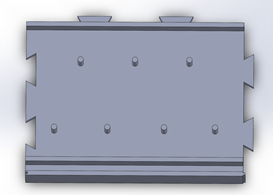
\includegraphics[width=\textwidth]{image/BodyModel6.png}
    \end{subfigure}
    \begin{subfigure}[b]{0.45\textwidth}
      \centering
      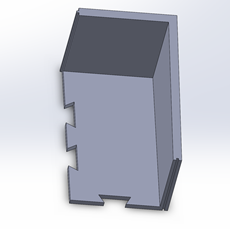
\includegraphics[width=\textwidth]{image/BodyModel7.png}
    \end{subfigure}
    \begin{subfigure}[b]{0.45\textwidth}
      \centering
      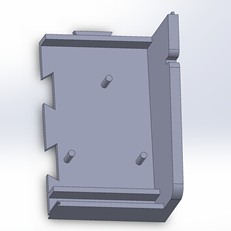
\includegraphics[width=\textwidth]{image/BodyModel8.png}
    \end{subfigure}
    \caption{}
    \label{fig:body_parts}
\end{figure}

As can be seen from these figures, each piece has been specially crafted to fit into each other like a puzzle. We can see the full arrangement of the assembled body in \textit{Figure \ref{fig:assembled_body}}.

\begin{figure}[h!]
  \centering
  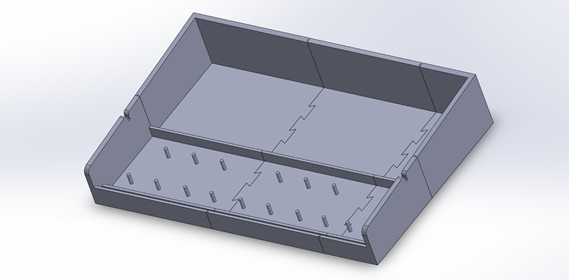
\includegraphics[width=0.9\linewidth]{image/AssembledBody.png}
  \caption{}
  \label{fig:assembled_body}
\end{figure}

This body allows for the keys to be elevated, keeps the bottom of the device level, maximizes the space for the electrical components, and protects the components inside. The front of the device starts at a max height of 63.42 mm and creates a 10 degree incline until the back of the device maxing out at 93.89 mm in height.

The cover or front panel of this device is 483x196.5 mm. There is absolutely no way to print this with our at home printer. Our front panel is shown in \textit{Figure \ref{fig:display_model}} and features five separate extruded cuts.

\begin{figure}[h!]
  \centering
  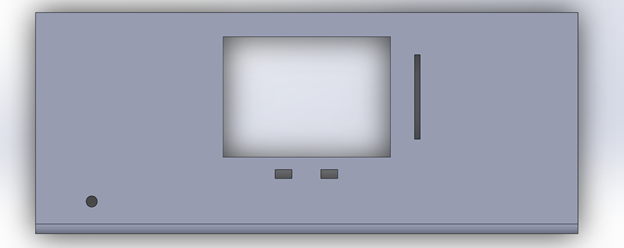
\includegraphics[width=0.9\linewidth]{image/DisplayModel.png}
  \caption{}
  \label{fig:display_model}
\end{figure}

In the center of the front panel is a 149 mm by 107 mm hole to house the seven inch capacitive touchscreen display. To the right of the display slot is a 5 x 75 mm slot designed to house the sliding potentiometer which will be used to control the volume of the device. Below the screen are the two holes where the octave up and octave down buttons will be placed and in the button left of the cover is where the audio jack for the user’s headphones to plug in will be installed.

Since the user interface will be controlled by a touch sensitive screen, we placed the slot equally spaced from the left and right of the cover to be able to equally treat left and right handed individuals. All the buttons and potentiometers surround closely as well for ease of use. The headphone jack was placed in its location because many over-ear headphone companies produce headphones with the wire extending from the left ear in hopes to avoid obstructing the right hand, which is the majority of the population’s dominant hand. Ultimately, everything needed a place and we felt these locations were the best fit.

When all the parts are connected and in place, the intended design of the body can be seen in \textit{Figure \ref{fig:final_model1}}. With the keys in place, the full assembly and design on the keyboard can be seen in \textit{Figure \ref{fig:final_model2}}.

\begin{figure}[h!]
  \centering
  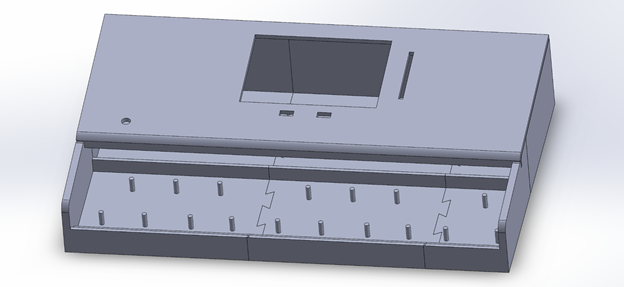
\includegraphics[width=0.8\linewidth]{image/FinalModel1.png}
  \caption{}
  \label{fig:final_model1}
\end{figure}

\begin{figure}[h!]
  \centering
  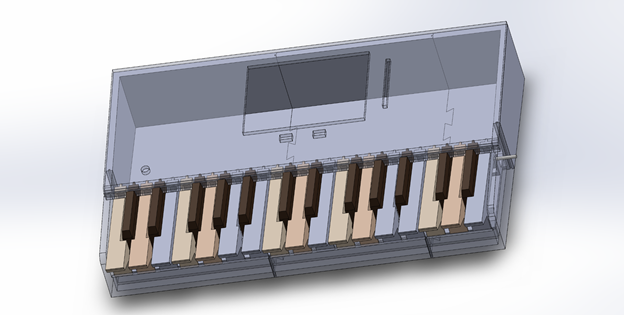
\includegraphics[width=0.8\linewidth]{image/FinalModel2.png}
  \caption{}
  \label{fig:final_model2}
\end{figure}

\subsubsection{DAW: Static}

Our DAW prototype was constructed without the use of the Electron UI-building environment. This
decision was motivated by the belief that creating the Electron application encompassed two
separate problems: the first was to create a fully functioning script, the second was to port that
script into the Electron application. By building the prototype outside of Electron, we aimed for
faster progress and less bottlenecking of the workflow by dealing with one smaller problem at a
time. Additionally, this decision expedited the debugging process by removing the need to load
the full Electron application every time we wished to monitor the progress of the build. Instead,
we could simply locate the HTML file in out directory and open it in a browser with a single click.

The first step in constructing the DAW was to establish all of the static elements, which include
the piano roll (which is displayed inside a horizontally-scrolling container), the guide keys, and
the menu buttons.

\paragraph{The piano roll} is the space in which the user can design their MIDI by adding,
moving, and removing notes. It appears as a rectangular space adorned with horizontal stripes. Each
white stripe corresponds to the vertical position that represents a white key on the keyboard, and
the same goes for the black stripes corresponding to black keys. Progressing upward in the pattern
of stripes is equivalent to progressing left to right on the keyboard. The guide keys follow a
similar format to the piano roll, with black and white stripes that visualize a piano keyboard
rotated 90 degrees counter-clockwise. Unlike the piano roll, however, the guide keys are much
shorter in width and remain as a static element outside (to the left) of the scroll container.
The stripes also display the name of the note to which they correspond. This allows the guide keys
to act as a reference for the user, so they can easily see which note each piano roll stripe
represents without having to count from the bottom. To serve this purpose properly, it is
imperative that the guide keys' stripes line up exactly with those on the piano roll.

This was achieved by building both assets using the same grid display class, given the name
"piano-container." In the CSS script, the piano-container class was styled as a grid display,
which established the appropriate pattern of black and white key items and set a standard gap of
one pixel between each key. The key items were then added as rectangular DIV objects with the
appropriate background color and a standard height of ten pixels. The guide keys were assigned an
additional class called "keys," which gave them a set width. Text was added in the center of each
DIV, labelling it by note. The piano roll was assigned the additional class "roll," which lowered
the opacity of the stripes to allow for better readability. The roll class also gave the piano roll
the absolute position attribute which allowed it to scroll within the scroll container.

At this stage of development, the dimensions of the screen upon which the DAW was to be displayed
were unknown. To proceed with prototyping at a timely pace, we made the width of the piano roll
flexible by reading the size of the window upon opening and setting the piano roll's width
attribute relative to the result. This means that the dimensions may not function properly if the
window is resized after opening, but this is not expected to be a problem because there will be
no way for the user to change the window size on the final keyboard.

\paragraph{The menu buttons} were added below the scroll container, separated into one group which is flush
left, and another which is flush right. The left button group deals with the state of the piano
roll; these buttons allow the user to save the state, reset it to its last save, and utilize undo and
redo functions to return the piano roll to a previous state. There is also a tempo button which
allows the user to select the tempo of playback. The right button group deals with the mode of
interaction. Depending on which of these buttons is selected, the users will be able to switch
between adding, deleting, moving, and stretching the notes on the roll. There are also play and
stop buttons that control playback, and a quantization button that can change the size and
positions the notes will snap to when editing. There is one additional button not included among
the menu buttons. This button exists on the far right of the piano roll, labelled with a plus sign.
It allows users to extend the piano roll so that they may create a longer melody.

\begin{figure}[h!]
  \centering
  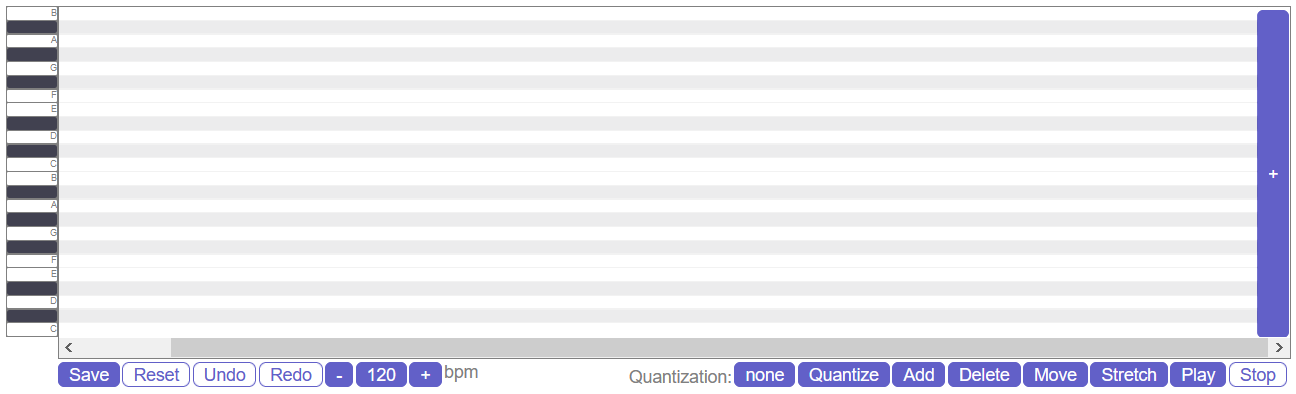
\includegraphics[width=\linewidth]{image/Static.png}
  \caption{A snapshot of the static assets of the DAW, the piano roll is empty}
  \label{fig:static}
\end{figure}

All UI buttons belong to the CSS class "ui," which gives them a uniform design. This class adds
several cosmetic elements to enhance the user experience by making interactions more visually
pleasing. The buttons have a periwinkle color and rounded corners to make them feel softer and
more polished than the default HTML button. They also expand in size and invert in color when
moused over to indicate they can be clicked. To make this transformation feel fluid, the transition
time has been set to 0.4 seconds, as opposed to the default 0 seconds which would have the buttons
snap immediately from one state to the next. Buttons that are disabled and cannot be clicked are
displayed at the standard size but with inverted colors.

\begin{figure}[h!]
  \centering
  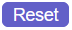
\includegraphics{image/StdUI.png}
  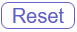
\includegraphics{image/HoverUI.png}
  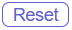
\includegraphics{image/DisabledUI.png}
  \caption{A sample of the styling of the menu buttons in their standard, hover, and disabled states respectively}
  \label{fig:ui_variations}
\end{figure}

The quantization and tempo control buttons take on a special structure. Clicking on either of
these buttons opens a drop-down menu from which the user may select a value. The tempo menu
provides options ranging from 30 to 300, but only lists multiples of 20. This is for the
convenience of the user; although they can select any tempo between 30 and 300 by incrementing or
decrementing using the “-“ and “+” buttons on either side of the tempo menu, the drop down allows
the user to skip through by larger units to expedite the process. The quantization button provides
options in the form of note lengths, with the largest being 1/1 and the smallest being 1/64. This
sets the size of the snap-grid on the piano roll relative to the size of a whole note. For example,
if the quantization was set to 1/1 and the user were to move a note, the note would snap to units
of 64 pixels on the horizontal axis because that is the length of a whole note. If the quantization
was set to 1/2, the note would snap to units of 32 pixels on the horizontal axis because that is
half the length of a whole note. Additionally, if the user were to click the “Quantize” button
after selecting a quantization value, all of the notes that are already on the piano roll would
immediately snap to the same units, as demonstrated in \textit{Figure \ref{fig:twinkle_quantized}}.

\begin{figure}[h!]
  \centering
  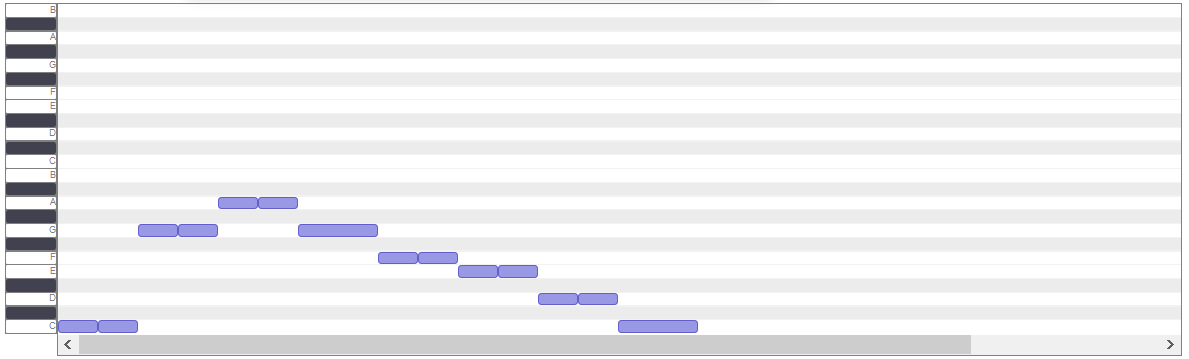
\includegraphics[width=\linewidth]{image/TwinkleOriginal.png}
  \caption{A piano roll displaying the default \textit{Twinkle, Twinkle, Little Star} melody}
  \label{fig:twinkle_original}
\end{figure}

\begin{figure}[h!]
  \centering
  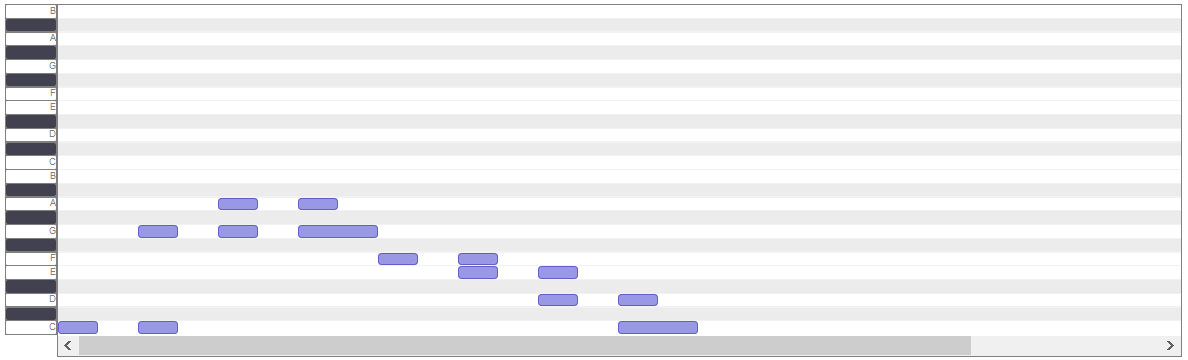
\includegraphics[width=\linewidth]{image/TwinkleQuantized.png}
  \caption{The same melody, now quantized to snap to half-note intervals}
  \label{fig:twinkle_quantized}
\end{figure}

The drop-down menus were achieved by adding a vertically-scrolling div containing all of the menu
options positioned so that the top option layers exactly over the button. This div has an initial
display attribute of “none,” so although all of its styling and position data are active, it is
neither visible for interactable. Pressing the button sets the menu display attribute to “block,”
which causes the menu to appear over the button and allows the user to interact. Clicking on a menu
item will update the piano roll settings and reset the menu display to “none,” making it disappear
and leaving only the button which will then be displaying the selected menu item.

\begin{figure}[h!]
  \centering
  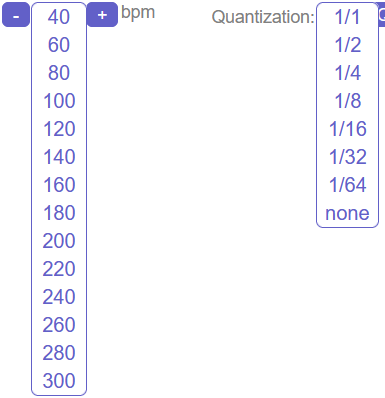
\includegraphics[width=0.4\linewidth]{image/Dropdowns.png}
  \caption{The expanded drop-down elements}
  \label{fig:dropdowns}
\end{figure}

UI buttons are enabled and disabled on a situational basis to prevent the user from interacting
with the application in an unintended manner. For example, the "Undo" button is disabled if no
edits have been made to the notes or if the user has reverted state using this button more than
the allotted number of times with no edits between. This prevents the user from reverting state
farther back than the original state upon opening. Similarly, the "Redo" button is disabled until
the "Undo" button has been pressed and disables again when any edits are made to the notes. This
prevents the users from redoing an undone state after an edit has been made, thus overwriting any
edits made since the "Undo" button was used. The "Reset" button is disabled only when the program
has just been opened or reset and no edits to the notes have been made since. This is not so much
to prevent the user from pressing it again, but more so to indicate to the user that resetting the
state again would be unnecessary and redundant. The "Play" button is only disabled when
the MIDI playback is active, while the "Stop" button behaves oppositely. Much like the "Reset"
button, this is primarily designed to indicate redundancy in an interaction, but also if the "Play"
button were to be pressed during MIDI playback, a second audio instance of the MIDI would begin
playing over top of the first. Finally, each of the mode buttons (Add, Delete, Move, and Stretch)
is disabled when its mode is active, to indicate to the user which edit mode the application is
currently running.

\paragraph{The MIDI notes} have been implemented in the form of buttons. These buttons have their own CSS
class, appropriately named "note," that give them a polished uniform look. For cohesion, the note
border is the same color as the buttons and the fill color is a slightly lighter shade. They also
have rounded corners to maintain the same polished feel as the menu buttons. The fill color
lightens when the note is hovered over to indicate to the user which element they are selecting.
This transformation could not be given a transition time like the menu buttons, though, because
extending the transition time would also extend the time the note takes to move around when being
dragged by the user.

The prototype opens with the first two lines of \textit{Twinkle, Twinkle, Little Star} as the default
melody. For each note, the program determines the position and dimensions based on its attributes
in the MIDI file. The heights of the notes are set equal to the height of the key template on the
piano roll so that they may align perfectly on top of the piano roll stripes. The vertical position
is assigned based on the note's pitch. MIDI pitch values start at 0 representing C in the -1 octave
and each integer increase represents an ascent of one diatonic step in the key of C. Our keyboard
prototype spans two octaves, with Middle C (C in the 4th octave) at its lowest extreme, so it
handles pitch values 60-83. To translate these pitch values into a vertical position, we
implemented the following formula:

\begin{equation} \label{note_vert}
  top_{note} = \Big((height_{note} + key\:gap) * 23 - \big((pitch_{note} -  60) * (height_{note} + key\:gap)\big)\Big)\;pixels
\end{equation}

Because the vertical position is measured in the number of pixels between the top of the parent
window and the top of the element, the first section of this formula $ (height_{note} + keygap) * 23 $
establishes that the search for the vertical position is based 23 keys from the top, which is
the lowest key on a two-octave keyboard. The second section $ (pitch_{note} -  60) * (height_{note} + keygap) $
shows that the base pitch is 60, and that the note's height above the the base key will be
proportional to the difference between the note's pitch and the base pitch in units equal to the
key height (maintaining the key gap in between).

The horizontal position is assigned based on the note's start time and the playback tempo. The
start time attribute in MIDI data is measured in seconds. Our prototype represents a whole note
with a width of 64 pixels, so the horizontal position of the note is determined by the following
formula:

\begin{equation} \label{note_vert}
  left_{note} = \frac{start\:time * 60}{tempo} * 64\;pixels
\end{equation}

The multiplication of the start time by 60 and subsequent division by the playback tempo
establishes the ratio between one second and one whole note. So through this, the number of
seconds is translated into a number of whole notes, and the final multiplication by 64 - the width
of a whole note - places the note at the corresponding beat on the piano roll.

The width of the note is similarly calculated based on the start time, end time, and tempo:

\begin{equation} \label{note_vert}
  width_{note} = \frac{(end\:time - start\:time) * 60}{tempo} * 64\;pixels
\end{equation}

The difference between the start and end time is converted to some decimal number of whole note
lengths, and this is translated into the width of the note in pixels.

\subsubsection{DAW: Functional}

\paragraph{Move}

Once the visual layout of the DAW had been established, we added interactivity in JavaScript. The
first function implemented was editing the note sequence by moving the notes, because this is
arguably the most used and therefore most important feature of a DAW. At this phase of development,
the methods of input were yet unknown - we intended to either use a single-touch touch screen or a
cursor controlled by arrow keys. The important thing to consider about how this affects UI design
is that moving an element in a 2D space requires a decent degree of freedom in the user inputs.
Single-touch touchscreens and arrow key cursors both provide limited input, but each lending to a
different style of interaction. To account for both possibilities, two versions of the note moving
function were developed: a click-and-drag version suited for touchscreen input and a
click-to-select/click-again-to-place version suited for arrow key input.

Rather than being on-click functions for the notes, each edit function is called with the notes as
its argument once the DAW has entered the corresponding edit mode. This is because the on-click
function of the notes must be edited at different points of interaction within the edit mode. At
its start, the click-and-drag move function sets the notes' on-mouse-down function to change the
on-mouse-move and on-mouse-up function. This means that the notes will not respond to cursor
movements unless the cursor has clicked and is holding over the note. The on-mouse-up function
resets the on-mouse-move and on-mouse-up functions to null, so once the mouse is released, the note
no longer responds to mouse movement. The activated on-mouse-move function will continuously edit
the position attributes of the note so that the note follows the cursor while snapping to valid
positions as determined by the quantization and available pitches.

The click-to-select version of the move function creates a boolean called "draggable," and each
note is linked to its own instance of draggable. Every note begins with draggable set to false,
indicating that the note will not move in response to cursor movements. When a note is clicked, its
draggable is switched – so on the first click, it will be switched to true. When draggable is true,
the on-click function sets the on-mouse-move function to move the note along with the cursor in the
same manner as the click-and-drag version. It also disables all other notes as well as the menu
buttons. This is to prevent the user from accidentally clicking a button and activating another
function before exiting the move function, which would likely cause interactions to clash in a
catastrophic way. Once the user has moved the cursor to the desired placement location, they can
click again – because the note follows the cursor, this will always result in the note being
clicked. This activates the on-click function a second time, which reverts draggable back to false
and proceeds to reactivate all other notes and buttons and revert the selected note’s on-mouse-move
function to null.

\begin{align} \label{move_horz}
  left_{note} = \max( & 0, \\
  & \min(left_{expand\:btn} - width_{note}, \\
  & x_{cursor} - (width_{guide\:keys} + left_{guide\:keys} - scroll) - \frac{width_{note}}{2})) \;pixels &
\end{align}

\begin{align} \label{move_vert}
  top_{note} = \max( & 0, \\
  & \min(23 * (height_{note} + key\:gap), \\
  & y_{cursor} - top_{piano\:roll} - \frac{width_{note}}{2})) \;pixels &
\end{align}

This first set of equations are used to move the note along with the cursor. In the following
segment, we will break them down line by line.

Both equations start with a $ \max $ function, with an argument of $ 0 $. This prevents the user from
dragging the note outside of the piano roll to the top or left. If the cursor were to go above or
left of the piano roll, the note will simply bump against the border and stop moving along that
axis until the cursor is back within the bounds. This is to prevent the user from losing the note
by accidentally dragging it outside of the piano roll and forgetting that it is out of bounds.

The second line of each equation serves the same purpose as the first, but this time setting the
bounds to the right and bottom of the piano roll, respectively. The first equation uses the left
border of the expand button as its right-most extreme. It also subtracts the width of the note
because this attribute sets the location of the left border of the note, so the prevent even part
of the note from going out of bounds, we must account for the whole length of the note. The second
equation uses $ 23*(height_{note} + key\: gap) $ as its minimum because that spaces the top of the
note 23 keys from the top. As we established in the initial loading of the notes, this is where the
base note is.

The third line of each equation moves the note to be centered under the cursor. The first equation
subtracts $ (width_{guide\:keys} +left_{guide keys} - scroll) $ from the cursor’s x position because
the cursor position is read in relation to the application window, but the note position is set in
relation to the piano roll. The sum of the guide key width and left position sets the base at the
right border of the guide keys - right where the scroll container starts. Then subtracting the
horizontal scroll of the piano roll counters the piano roll’s offset relative to the scroll
container. Finally, half the width of the note is subtracted to put the cursor over the center. The
second equation accounts for the piano roll offset by subtracting the roll’s top position, then
also subtracts half the note’s height to put the cursor over the center.

Next, we will discuss how the function snaps the notes to the quantization grid. After the notes
have been moved to meet the cursor, their positions are once again altered to only move in units of
a specified number of pixels.

\begin{equation} \label{vert_snap}
  left_{note} = \round(\frac{left_{note}}{64 * quantization}) * 64 * quatization \;pixels
\end{equation}

\begin{equation} \label{horz_snap}
  top_{note} = \round(\frac{top_{note}}{height_{note} + key\:gap}) * (height_{note} + key\:gap) \;pixels
\end{equation}

This second set of equations rounds out the note’s position under the cursor to an integer number
of the accepted units, then multiplies that integer by the size of the unit to get the nearest
valid note position. For the horizontal axis, the acceptable units are $ 64 * quantization $
because 64 is the width of a whole note, and the quantization is the desired note value (fraction
of a whole note) to snap to. For the vertical axis, the unit is $ height_{note} + key\:gap $ to
keep the notes in line with the rows in the piano roll.

\paragraph{Stretch}

The stretch function is similar to the move function in both mechanics and importance. Because of
these similarities, the stretch function also has the click-and-drag and click-to-select variations.

The overall mechanics are the same. The click-and-drag sets the note to respond to mouse movement
by editing the on-mouse-move function through the on-mouse-down function. It then releases the note
from movement by setting the on-mouse-move function to null through the on-mouse-up function. The
click-to-select gives every note an instance of the Boolean “stretchable” which defaults to false.
The note’s on-click function switched stretchable, then checks stretchable’s state. If stretchable
has been switched to true, all other buttons are disabled and the note’s on-mouse-move function is
set move it in response to the cursor. If stretchable has been switched to false, the on-mouse-move
function returns to null and all other buttons are enabled once again.

This function also uses similar math to determine the note’s new width.

\begin{align} \label{stretch}
  width_{note} = \max( & 64 * quantization, \\
  & \min(left_{expand\:btn} - left_{note}, \\
  & x_{cursor} - (left_{note} + width_{guide\:keys} + left_{guide\:keys}))) \;pixels &
\end{align}

Once again, the first line uses a $ \max $ function to set the minimum extreme. The smallest a note
can be is one quantized unit, which we have established to be $ 64 * quantization $. The second
line sets the maximum extreme. To keep the note from expanding beyond the bounds of the piano roll,
the largest allowable with is equal to the distance between the note’s left bound and the piano
roll’s right bound, which we can see to be $ left_{expand\:btn} - left_{note} $. The third line
changes the width based on the cursor’s distance from the start of the note. Once again, the left
position and width of the key guide are accounted for because the cursor and the note are relative
to different windows due to the note being a child element of the scroll container. Because we are
dealing with differences, unlike the move function, the stretch function does not have to counter
the offset caused by the scroll.

\begin{equation} \label{stretch_snap}
  width_{note} = \lceil\frac{width_{note}}{64 * quantization}\rceil * 64 * quantization \;pixels
\end{equation}

Unlike the move function, rather than rounding the updated note width to determine the number of
units, the stretch function takes the ceiling. This is simply to enhance the look and feel of the
movement. Rounding in the move function allows the note to appear to the left or right of the
cursor. Taking the ceiling in the stretch function ensures that the width is always greater than or
equal to the distance between the cursor and the start of the note. This means the cursor will
always be encompassed by the note.

\paragraph{Add}

The remaining edit functions are comparatively simple. The add function sets all note on-click
functions to null to prevent from spawning a note directly on top of another note. It then sets the
on-click function of the piano roll itself to spawn a new button when a blank area on the roll is
clicked. The new button is given the “note” class so it will be stylized uniformly to the other
notes. The note is then appended as a child of the scroll container so that it will scroll with the
piano roll and maintain its position relative to other notes. Its width is set equal to one
quantized unit, and its position is determined using the same technique as the move function. First
it is centered over where the mouse was clicked, then it snaps to the nearest valid position.

\paragraph{Delete}

The delete function is the simplest among the edit functions. It simply sets the notes’ on-click
function to JavaScript’s element remove method. When a note is clicked, it is removed from the
application, along with all references to it.

\paragraph{Save}

Next, we will discuss the state functions. These functions handle the “state” of the piano roll,
meaning its current configuration of notes. The save function saves the current melody sequence
into memory; when the piano roll is reset, it will revert to the most recently saved state. The
application preserves the state by reversing the calculations done to place the notes initially,
thus turning the piano roll back into MIDI data.

\begin{equation} \label{get_pitch}
  pitch_{note} = 60 + \frac{(height_{note} + key\:gap) * 23 - top_{note}}{height_{note} + key\:gap}
\end{equation}

\begin{equation} \label{get_start}
  start\:time_{note} = \frac{left_{note}}{64} * \frac{tempo}{60}
\end{equation}

\begin{equation} \label{get_end}
  end\:time_{note} = start\:time_{note} + \frac{left_{note}}{64} * \frac{tempo}{60}
\end{equation}

The pitch of the note is based at 60 on the lowest key located at
$ (height_{note} +key\:gap) * 3 $. Subtracting the top position of the note shows the pixel
distance between the selected note and the base note. This is then divided by the unit size of the
note (plus key gap) to determine the number of keys between the note and the base note. This number
translates directly to the integer difference between the selected note’s pitch and the base pitch
60.

The start time of the note is calculated first by converting the pixel measurement left position
of the note into some decimal number of whole notes. The tempo is then converted from beats per
minute to beats per second. The two converted numbers are multiplied to get the start time in
seconds.

The end time of the note is offset by the start time, then uses the same pixel-to-note-value and
tempo-to-time conversions to determine the duration.

\paragraph{Reset}

The reset function loads the saved state and converts the MIDI data back into a piano roll
configuration. To start, it deletes all of the existing notes. Then it simply repopulates the piano
roll using the same steps the application originally used to convert the default melody when it was
initially opened.

\paragraph{Undo}

Whenever an interaction is made in any edit mode, before any changes are made to the notes, the
 current state is saved to a queue in the application’s backend. This process of saving the state
 uses the same conversions as the save function. When the undo function is called, it pops a state
 off the queue and converts the MIDI data back into a piano roll configuration using the same
 conversions used when the piano roll was initialized with the default melody. Additionally, when
 states are saved to the queue and the queue is at length 10, it will shift before pushing the new
 state into the queue. This limits the user’s number of successive reversions to 10, after which
 the undo button will be disabled until new edits are made to repopulate the queue. This
 limitation was imposed to prevent the application from having to store an infinite number of
 states into memory. Because we are operating on standalone hardware, memory is limited and must be
 consumed shrewdly.

\paragraph{Redo}

Whenever the undo function is called, before the piano roll state is reverted, it is saved to a
second queue. This queue behaves much like that used by the undo function. When the redo function
is called, it pops a state off and translates it onto the piano roll. However, whenever any edit is
made besides a call on the undo function, the redo queue empties itself and is disabled until the
undo function is called.

\paragraph{Expand}

The expand button is the button at the end of the piano roll labelled simply with a “+.” Clicking
this button edits the piano roll attribute to increase its width by 256 pixels. This pixel width
is equal to four whole notes, or one bar of music.


\paragraph{Play}

Finally, we get to discuss MIDI playback. The playback process begins by reading the piano roll
back into a MIDI sequence using the same methods as the state functions. The application then
creates an audio node with an appended gain node. It iterates through the MIDI data, and for each
note creates an oscillator that outputs a square wave tone at the corresponding frequency. MIDI
pitch values do not translate directly into note frequencies, however, so this must be done through
the following calculation:

\begin{equation} \label{get_frequency}
  f = 2^{\frac{pitch - 69}{12}} * 440 \;Hz
\end{equation}

While MIDI pitches are based around C4 = 60, frequencies are centered around A4 because it has the
simplest frequency value, at 440 Hz. This explains the presence of both 69 (the MIDI pitch value
for A4) and 440. This sequence of operations represent moving the base to A4, and then converting
MIDI units to frequency units. The 12 represents semitonal units, so the division of 12 shows the
difference in pitch is being converted to some number of semitones above A4. The base 2 is a
conversion to the number of octaves above A4. As we saw in the research section on harmonics, the
frequency difference between octaves of the same note is not constant. Instead octave frequencies
increase exponentially by base 2.

Once the frequency of the oscillator is set, it is scheduled to start and stop directly according
to the start and stop times given in the MIDI data. Though each start and stop is offset by one
second. This is to make sure the application has enough time to finish creating all the oscillators
before it begins playing audio. If the offset is removed, the audio player will occasionally cut
off the first half-second of melody.

While playback is active, the “Play” button is replaced by a “Pause” button that suspends the audio
node without closing it. Pressing “Play” again will resume the melody right where it left off.

If an audio node is active, there is also the option to stop playback using the “Stop” button. This
function will close the audio node entirely, setting playback back to the start if the user were to
press play again.


\subsection{Testing}

\subsubsection{DAW}

Because there is no way of measuring performance of the DAW, testing it was difficult. Simply, the
quality of the DAW is largely based on the look and feel of it, as well as its ability to handle
edge cases. However, there is no way of simply knowing what edge cases there are, especially for
an application with so many moving parts. Our ultimate method of testing was to allow team members
Brian and Sam, who have sufficient experience producing music using DAWs, to experiment with its
functionality and try to find edge cases by using unconventional methods.

\subsubsection{Keyboard}

\blindtext

\subsubsection{AI}

\blindtext

\subsection{Evaluation}

\subsubsection{DAW}

After receiving feedback from our test group, we have found that the overall look and feel of the
DAW has achieved sufficient polish. The UI design is clean and the fluidness of interactions is
comparable to other simple browser-based DAWs, such as Soundtrap.

\begin{figure}[h!]
  \centering
  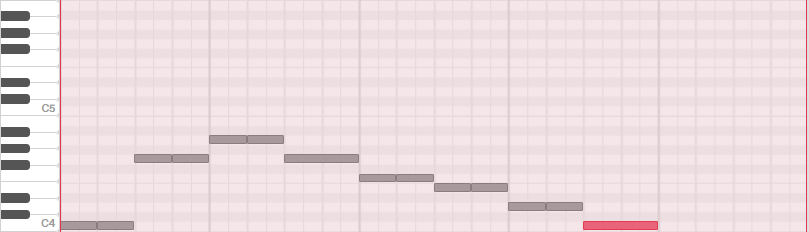
\includegraphics[width=\linewidth]{image/Soundtrap.png}
  \caption{A snapshot of the Soundtrap MIDI editor displaying the \textit{Twinkle, Twinkle, Little Star} melody.}
  \label{fig:soundtrap}
\end{figure}

Our test group did manage to find edge cases regarding the snap-to-grid functionality in the use
of the move edit mode. Because the snap moves the note after centering it under the mouse, if the
quantized unit size is large enough, the note is occasionally not under the cursor. In the
click-to-place version of the move function, if the user clicks in this condition, the note will
release its on-mouse-move function making it static but not exiting the move mode. When this
happens, the user will no longer be able to interact with any of the notes until they click the
note they had originally selected. If the user cannot remember which note that is, they can get
stuck on a frozen piano roll. The final iteration of this project will address this issue by only
making the note snap to position if the cursor is within a note-width of a grid marker.

Other test sessions found that the transition of states between the state functions is flawed.
Occasionally, the "Undo" and "Redo" buttons would disable when they should have been enabled. This
issue will be addressed in the final version by refactoring the flow of saved states between the
functions.

Our test group also remarked on quality-of-life features that could be added to improve the user
experience. For example, a time scroller which allows the user to manually skip backward and
forward in MIDI playback. Another suggestion was to have the notes and guide keys play a
one-second sample of the note when clicked so that the user can get an idea of the melody they
are constructing. It was also suggested that the piano roll could include vertical markers that
show where each quarter-/half-/whole-note increment lies, similar to what Soundtrap implements in
\textit{Figure \ref{fig:soundtrap}}.

\begin{figure}[h!]
  \centering
  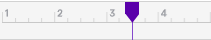
\includegraphics{image/Scroller.png}
  \caption{An example of a DAW time scroller}
  \label{fig:scroller}
\end{figure}

\subsubsection{Keyboard}

\blindtext

\subsubsection{AI}

\blindtext
